\chapter{极限精度梯度压缩方法}
考虑到梯度数据普遍较小,绝大部分数据绝对值在0~1之间这样特点,如表~\ref{tab:resnet50_1iter_grad_fabs}所示。在resnet50网络中,每次迭代需要更新155个tensor的梯度,表中展示了在第一次迭代中各个tensor最大绝对值所处的范围。可知仅考虑每个tensor中最大绝对值情况下,53.55\%的tensor中最大绝对值在0~1之间;41.29\%的tensor中最大绝对值在1~10之间;仅有5.16\%的tensor中最大绝对值在10~50之间。
\begin{table}[htb]
\centering
\noindent\begin{minipage}{0.65\textwidth}
\centering
\caption{resnet50第一次迭代中各层梯度最大绝对值分布}
\label{tab:resnet50_1iter_grad_fabs}
\begin{tabular}{p{2.5cm}p{2.5cm}p{2.5cm}}
\toprule[1.5pt]
梯度绝对值 & 数量 & 占比(\%) \\\midrule[1pt]
0~1.0 & 83 & 53.55\\
1.0~10.0 & 64 & 41.29\\
10.0~50.0 & 8 & 5.16\\
\midrule[1pt]
\end{tabular}
\end{minipage}
\end{table}

随着训练的进行,网络逐渐趋向于稳定,梯度数据的波动范围更小,更集中于0~1之间。如表~\ref{tab:resnet50_21iter_grad_fabs}所示。在第21次迭代中绝对值在0~1之间的梯度占比为74.84\%,1~10和10~50之间的梯度数量相对减少。可知在后面训练的迭代中梯度数据的绝对值将更加集中于0~1之间。故本章希望针对梯度数据这一特点,使用更少比特位表示梯度。通过减少梯度数据的表示位,可减少分布式训练程中的同步数据量,进而提高分布式系统的可扩展性和训练效率。
\begin{table}[htb]
\centering
\noindent\begin{minipage}{0.65\textwidth}
\centering
\caption{resnet50第21次迭代中各层梯度最大绝对值分布}
\label{tab:resnet50_21iter_grad_fabs}
\begin{tabular}{p{2.5cm}p{2.5cm}p{2.5cm}}
\toprule[1.5pt]
梯度绝对值 & 数量 & 占比(\%) \\\midrule[1pt]
0~1.0 & 116 & 74.84\\
1.0~10.0 & 37 & 23.87\\
10.0~50.0 & 2 & 1.29\\
\midrule[1pt]
\end{tabular}
\end{minipage}
\end{table}

本章希望在不影响神经网络训练精度的情况下,尽可能减少梯度数据所需的比特位数,为进一步减少分布式通信开销,提高分布式系统可扩展性和训练效率提供数据压缩方法。本章将主要介绍梯度压缩的思路与实现方法,以及对应压缩方式在图像分类和物体检测网络中的训练精度。通过其与原始的训练精度对比,说明对应压缩算法的有效性和适用范围。本章共提出两种极限精度梯度压缩EPGC方法:9比特梯度压缩方法和8比特梯度压缩方法,这两种算法均能保证分类网络训练精度达到原始浮点数训练相同精度。后面将详细分析相关实验结果。
\section{引言}
根据第二章内容可知,分布式训练过程中同步开销的大小对系统的可扩展性和训练效率有至关重要的影响。在不影响训练精度的情况下,将梯度尽可能地压缩则可减少同步开销,提高分布式系统的可扩展性和训练效率。本章将介绍探索梯度压缩方法的思路与具体实现方法,以及各个压缩方式下分类网和物体检测网络的最终收敛精度。

由第三章LPDU算法实现可知,基于horovod要实现新的数据压缩方法,则需在MPI中新增一个数据类型来解析该压缩数据,并实现一个该数据类型的求和函数供MPI调用。为快速验证本文提出的梯度压缩方法对神经网络训练精度的影响,本章提出的梯度压缩方法均通过对FP32浮点数或半精度浮点数对应比特位清零的方式来模拟对应的压缩方法。该模拟方法可避免对MPI的改动,使得本节提出的压缩方法能够快速得到验证。下面将对本节探索出的两种EPGC方法:9比特梯度压缩方法和8比特梯度压缩方法进行详细介绍。
\section{9比特梯度压缩算法}
根据上一章LPDU算法可知,BF16数据格式相对于原始FP32数据而言,去除了浮点数尾数中的后16比特位,仅保留7位有效比特位。本压缩算法根据这一思路,在BF16数据基础上,进一步减少尾数有效位,在保证训练精度情况下,尽可能减少尾数比特位,以减少分布式同步中的通信量。

\subsection{9比特压缩方法实现}
\begin{figure}[htp]
\centering
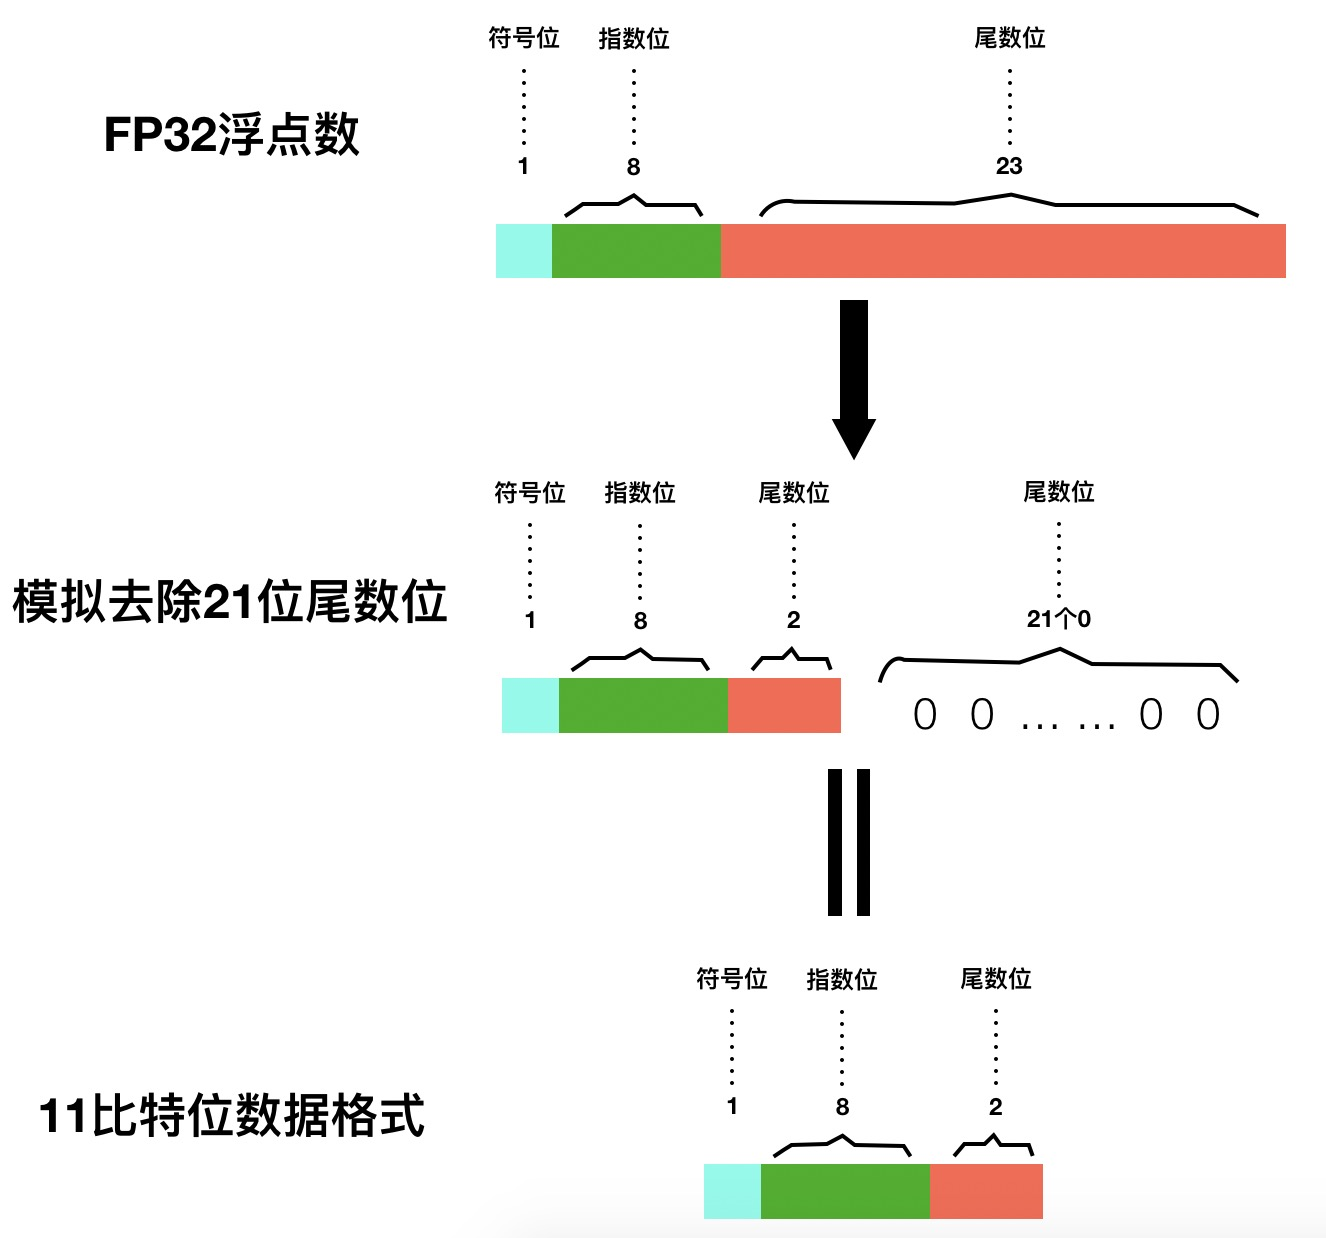
\includegraphics[width=10cm]{simulate_11bits}
\caption{模拟11比特数据表示示意图}
\label{fig:simulate_11bits}
\end{figure}
本节通过对原始FP32浮点数尾数位置零的方法模拟这种压缩方法。如在FP32浮点数基础上仅保留两位有效尾数位,形成11比特的数据格式,可通过将FP32浮点数的低21位清零达到相同效果,如图~\ref{fig:simulate_11bits}所示。可知低21比特位清零后的浮点数等效于11比特位数据格式所表示数据。

使用这种模拟方法,本文逐渐减少尾数比特位,并在对应比特位中使用图像分类和物体检测领域经典的网络,来验证该压缩方法的有效性和适用范围。最终发现在去除所有尾数情况下,仅使用9比特梯度压缩算法即可保证分类网的训练精度,故本节提出了适用于图像分类网络的9比特梯度压缩方法;但该梯度压缩方法在物体检测网络中则对网络训练精度有较大影响。

\subsection{9比特压缩方法实验分析}
通过这种模拟方法,本文分别得出使用11比特,10比特,9比特情况下,压缩算法对分类网和物体检测网的影响。分类网以resnet50为例,物体检测网络以SSD为例。经实验验证:在同步梯度数据时仅保留两比特位的尾数情况下,分类网也可收敛到原始浮点数梯度相同精度。在11比特有效位基础上,继续减少尾数位,保留1位尾数、去除所有尾数位情况下,在分类网上均能达到理想收敛精度。在去除所有尾数位仅使用9比特数据表示梯度情况下,resnet50的收敛曲线如图~\ref{fig:simulate_9bits_acc}所示。

\begin{figure}[htp]
\centering
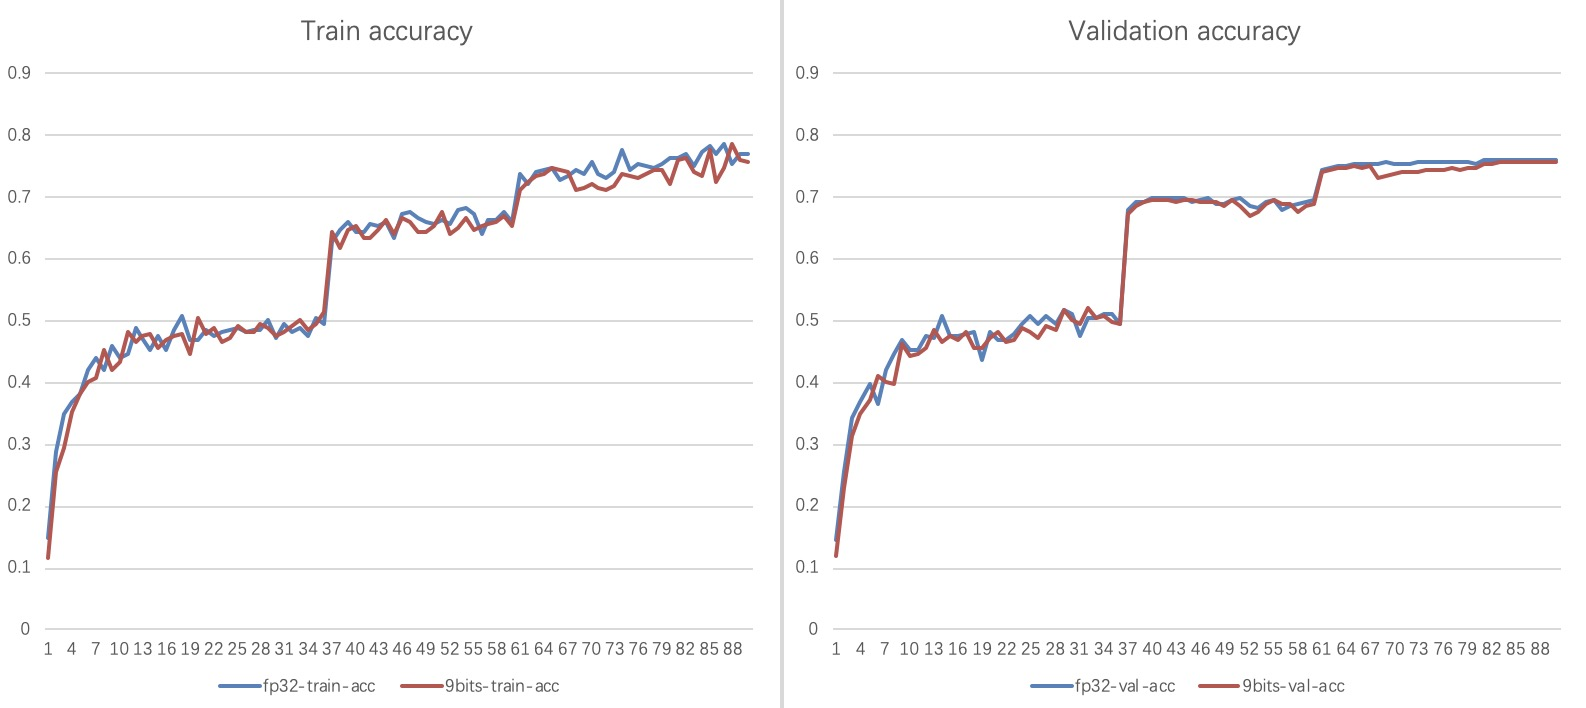
\includegraphics[width=13cm]{simulate_9bits_acc2}
\caption{9比特梯度压缩方法与原始浮点数表示训练精度曲线}
\label{fig:simulate_9bits_acc}
\end{figure}

在SSD中使用该压缩算法训练,其精度与原始网络训练精度差距较大,在保留2位尾数,1位尾数,去除所有尾数情况下,SSD的收敛曲线如图~\ref{fig:simulate_9bits_ssd_acc}所示。可知,在11比特压缩方法下,SSD的收敛精度已经与原始浮点数训练精度有一定差距。说明物体检测网络对梯度精度要求要高于图像分类网络。随着尾数位的不断减少,SSD的收敛精度也越来越低。
\begin{figure}[htp]
\centering
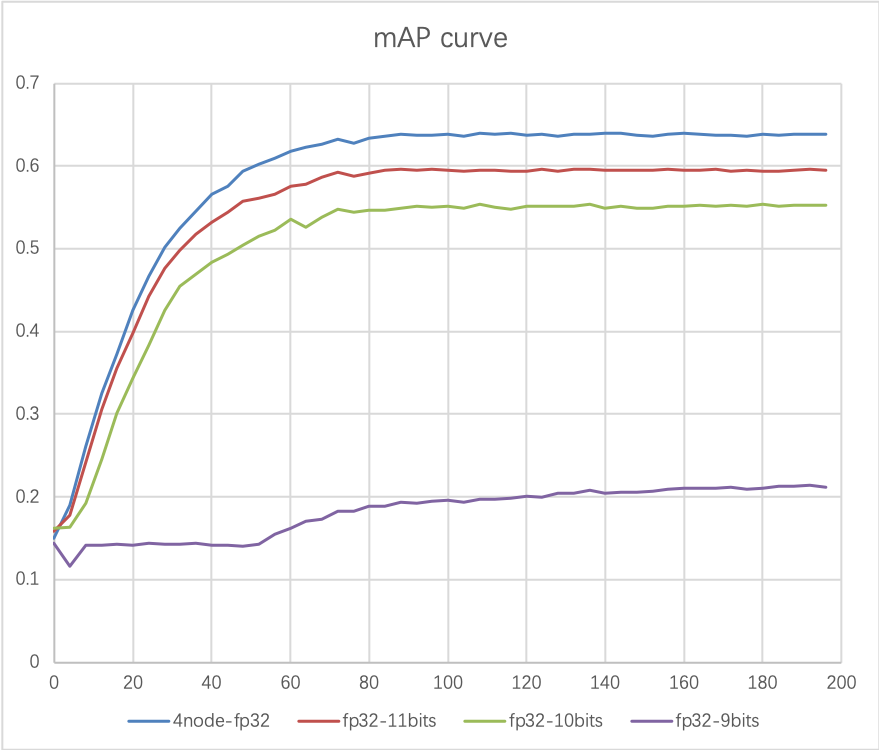
\includegraphics[width=12cm]{simulate_9bits_ssd_acc}
\caption{SSD在不同比特压缩算法下mAP曲线}
\label{fig:simulate_9bits_ssd_acc}
\end{figure}

保留2位尾数,1位尾数,不保留尾数情况下,resnet50与SSD在验证集准确率如表~\ref{tab:simulate_11_10_9bits_acc}所示。所有结果均在4节点8实例配置下训练得到。由表~\ref{tab:simulate_11_10_9bits_acc}可知,在原始浮点梯度基础上,仅保留2位尾数,1位尾数,不保留尾数情况下,resnet50网络精度与原始浮点数梯度精度相差<0.3\%。说明在误差允许范围内,在分类网中仅使用9比特数据(1个符号位,8个指数位)表示梯度即可满足训练精度要求。通过去除浮点数中所有尾数位的方法可在不影响神经网络训练精度前提下减少分布式同步开销,提升分布式系统的可扩展性和训练效率。而物体检测网络对梯度精度要求较高,本节提出的压缩方法则不适用于物体检测网络的训练。

\begin{table}[htb]
\centering
\noindent\begin{minipage}{0.6\textwidth}
\centering
\caption{不同尾数位下resnet50与SSD准确率}
\label{tab:simulate_11_10_9bits_acc}
\begin{tabular}{p{2cm}p{2.5cm}p{2.5cm}}
\toprule[1.5pt]
有效尾数位 & resnet50 acc(\%) & SSD mAP(\%) \\\midrule[1pt]
FP32 & 76.12 & 64.00 \\
2 & 76.08 & 59.66 \\
1 & 76.01 & 55.33 \\
0 & 75.87 & 21.36 \\
\midrule[1pt]
\end{tabular}
\end{minipage}
\end{table}
为找出适用于物体检测网络的压缩方法,下一步将基于11比特梯度压缩方法,进一步增加尾数位,对物体检测网络进行分布式训练,直到找到在保证网络收敛精度的前提下,所需的最少比特位。

\section{8比特梯度压缩方法}
由本文第二章可知,半精度浮点数也可用于训练神经网络,也能保证网络的训练精度与原始浮点数训练一致。半精度浮点数与BF16数据格式相比,少了3个指数位,仅5个指数位。根据上一节9比特梯度压缩方法可知,在仅保留2位,1位尾数或不保留尾数位情况下,均能保证图像分类网络训练精度与原始浮点数训练精度在误差允许范围内。本节结合半精度浮点数特点,本节提出8比特梯度压缩方法:在半精度浮点数基础上,去除16位半精度浮点数中低8位尾数,仅保留两个有效尾数位,使用8比特数据表示梯度,以此将梯度压缩成单字节数据。
\subsection{8比特压缩方法实现}
为快速验证本节所提出的梯度压缩方法的有效性,本节通过将半精度浮点数特定尾数位清零的方式模拟该压缩方法。原理如图~\ref{fig:simulate_8bits}所示。可知将FP16格式数据低8比特位清零后的半精度浮点数等效于8比特位数据格式所表示数据。

本文分别在resnet50和SSD训练中使用这种8比特梯度压缩方法,通过比较网络与原始浮点数训练的收敛精度来验证该压缩方法的有效性和适用范围。发现本节提出的8比特梯度压缩方法在分类网训练中不会对网络精度造成影响,在物体检测网络中则稍有影响。
\begin{figure}[htp]
\centering
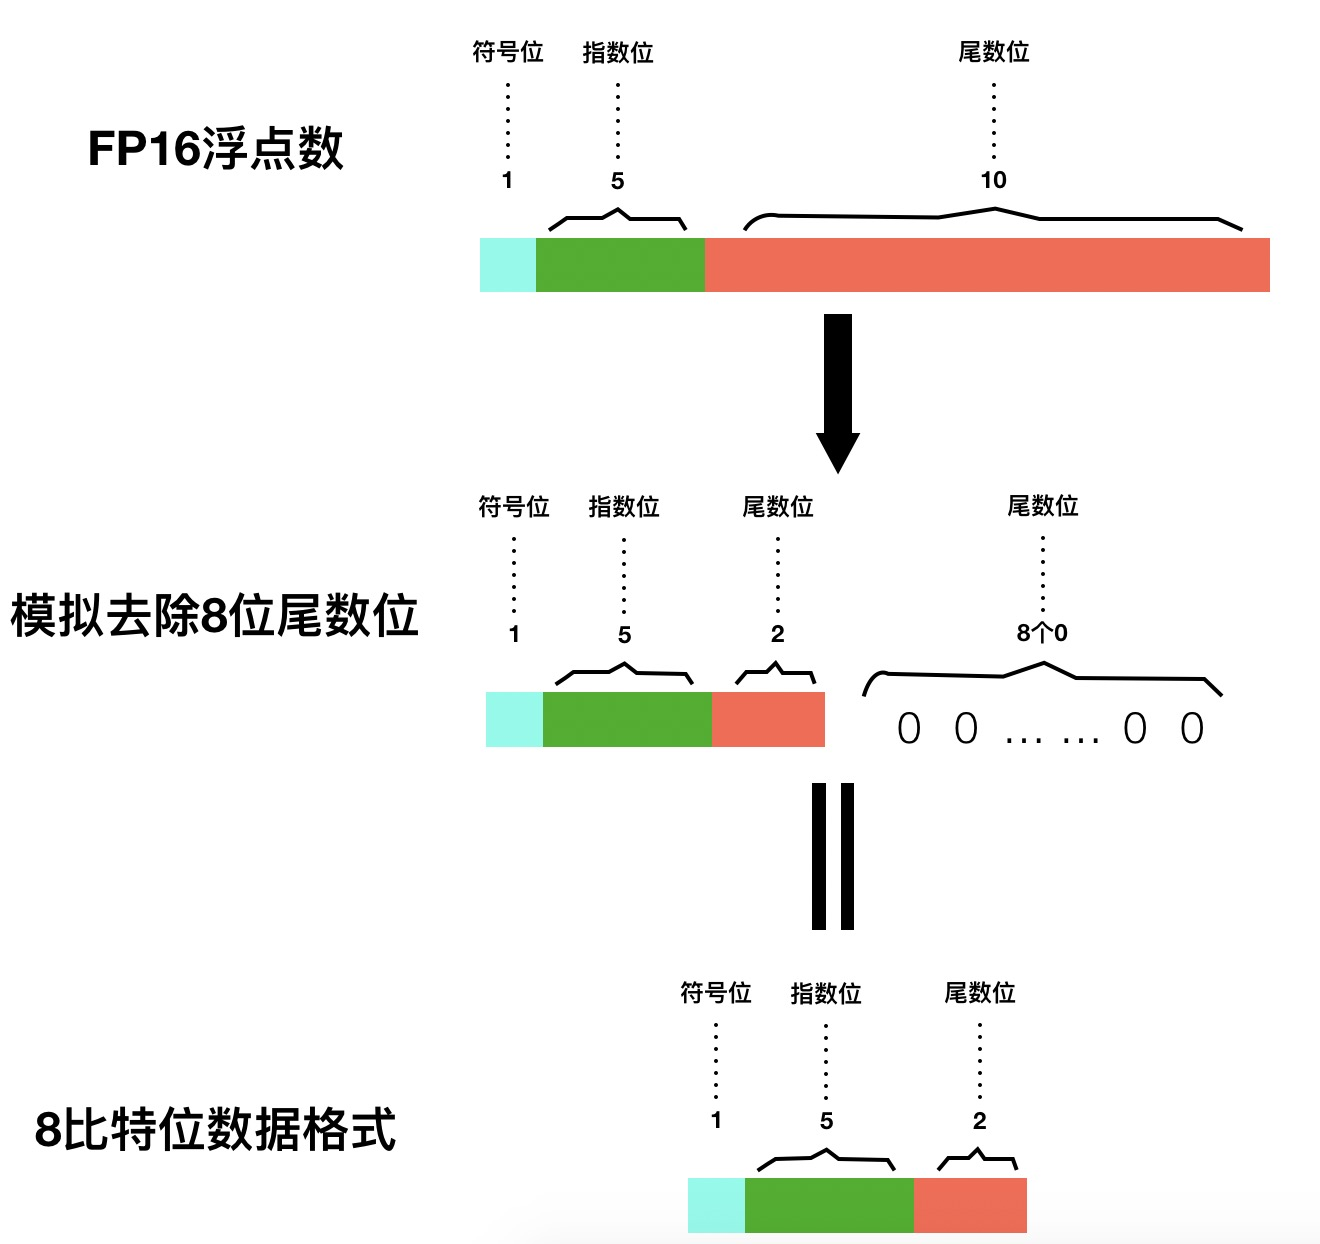
\includegraphics[width=10cm]{simulate_8bits}
\caption{模拟8比特数据表示示意图}
\label{fig:simulate_8bits}
\end{figure}

\subsection{8比特压缩方法实验分析}
在4节点8实例情况下,使用该方法将梯度数据压缩成单字节数据,resnet50的收敛曲线如图~\ref{fig:simulate_8bits_acc}所示。可知本节提出的8比特梯度压缩方法同样能达到原始训练精度:76.1\%,说明本节提出的压缩方法可在不影响分类网络精度情况下,减小分布式训练神经网络中的通信量,从而提升分布式系统的可扩展性和训练效率。
\begin{figure}[htp]
\centering
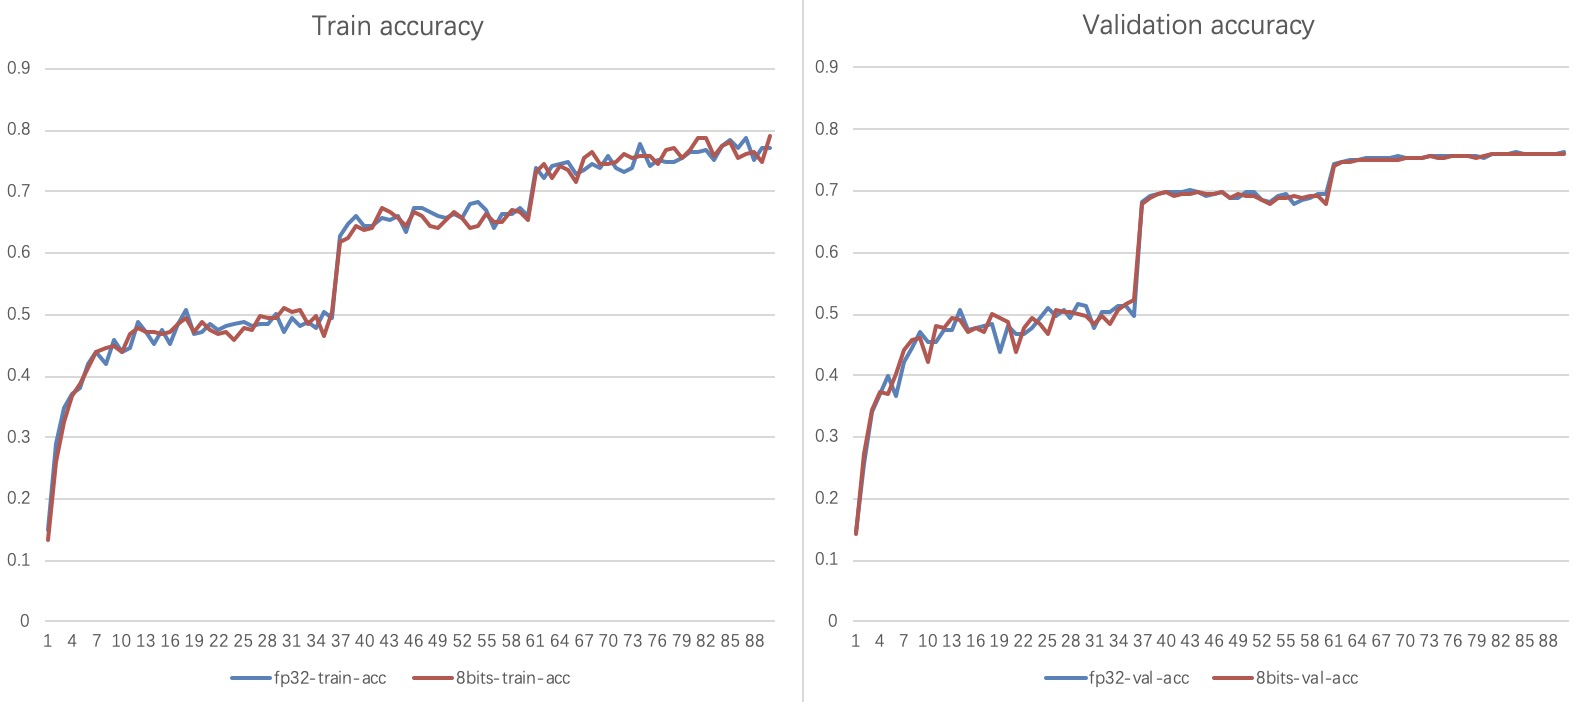
\includegraphics[width=13cm]{simulate_8bits_acc2}
\caption{8比特位梯度压缩方法与原始浮点数表示resnet50精度曲线}
\label{fig:simulate_8bits_acc}
\end{figure}

物体检测网络SSD在该压缩方法下mAP曲线如图~\ref{fig:simulate_8bits_ssd_acc}所示。可知SSD网络在本节8比特梯度压缩方法下最终mAP为59.78\%,与原始浮点数训练的结果:64.00\%差距较大。造成SSD训练精度的损失来自于尾数位精度的降低,其原因与9比特梯度压缩方法造成SSD训练精度下降的原因相同。说明本节提出的8比特梯度压缩方法在图像分类网络训练中不会对训练精度造成影响,可将该压缩算法用于分布式训练分类网,以提升训练效率。但因为物体检测网络对梯度精度要求较高,本节提出的8比特梯度压缩算法不能保证物体检测网络的训练精度,不适用于物体检测网络。
\begin{figure}[htp]
\centering
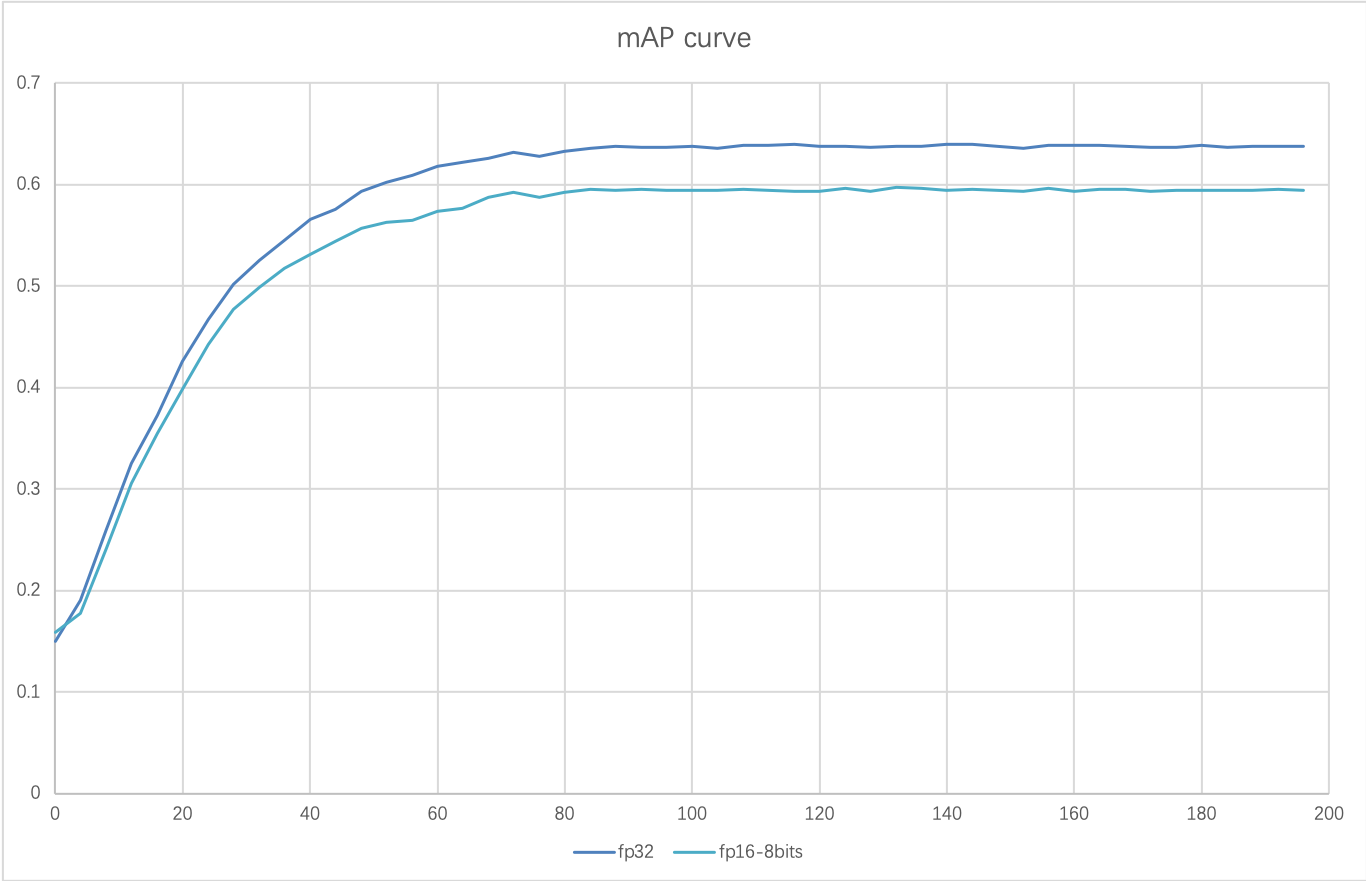
\includegraphics[width=12cm]{simulate_8bits_ssd_acc}
\caption{8比特位梯度压缩方法与原始浮点数表示SSD mAP曲线}
\label{fig:simulate_8bits_ssd_acc}
\end{figure}

同时,根据上一节提出的9比特压缩方法可知,可进一步在半精度浮点数上减少尾数位或去除所有尾数位,极限情况下仅使用6比特数据表示梯度。下一步将对这种可能的6比特梯度压缩方法在分类网络中进行尝试验证,通过比较该压缩方法下分类网的最终收敛精度与原始收敛精度的差异,说明该压缩算法对分类网精度的影响,从而确定该压缩算法应用于分类网络的可行性。

另一方面,对于本节8比特梯度压缩方法对物体检测网络造成精度下降的问题,下一步将在8比特压缩方法基础上,逐步增加尾数位,分别训练物体检测网络,直到物体检测网络训练精度达到原始浮点数训练精度为止。
\section{本章小结}
本章基于减少分布式训练神经网络通信开销,提高分布式系统的可扩展性和训练效率的目的,希望通过减少梯度数据比特位的方法来减少通信数据量,提出两种极限梯度压缩方法:9比特梯度压缩方法和8比特梯度压缩方法。经验证本章提出的两种压缩方法在resnet50网络中均能达到训练精度要求,说明这两种压缩方法应用于分类网络的可行性;也可看出物体检测网络对梯度精度要求较高,本章提出的两种压缩算法不适用于物体检测网络。下一步主要有两方面工作:1.基于8比特梯度压缩方法,继续减少尾数位,极限情况下仅使用6比特数据传输梯度,将其应用于分类网的训练,通过比较其训练精度与原始训练精度的差异,验证这种压缩算法的可行性;2.针对8比特梯度压缩方法在物体检测网络上造成精度损失的问题,基于8比特梯度压缩方法,逐渐增加尾数位,直至其在物体检测网络中的训练精度达到原始浮点数训练精度为止。







